\chapter{Käyttötapaukset}

\section{Käyttötapauskaavio}
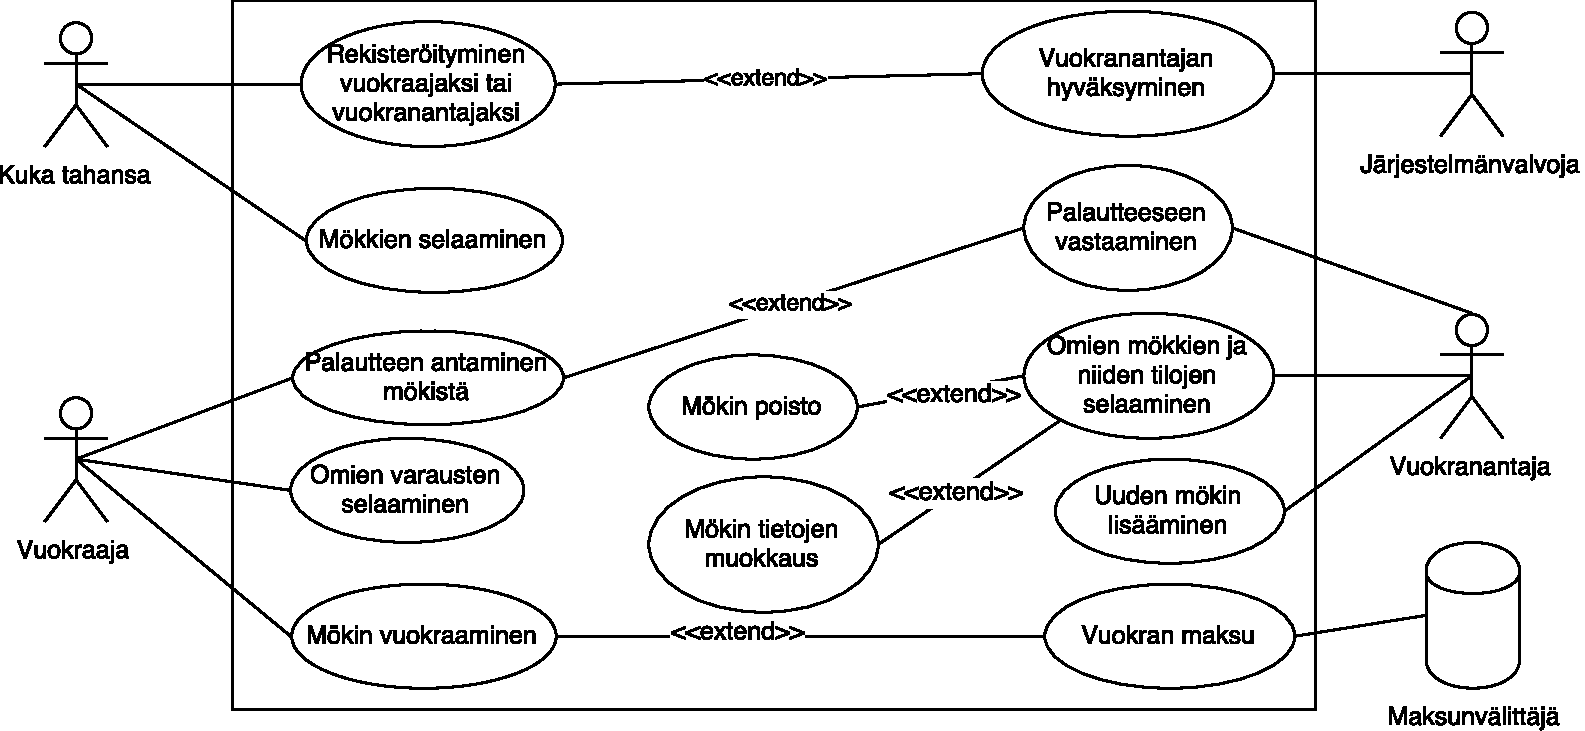
\includegraphics[width = 14cm]{./diagrams/drawio_usecase.pdf}

\section{Käyttäjäryhmät}

\subsection*{Kuka tahansa}
Kenellä tahansa tarkoitetaan kaikkia rekisteröityneitä ja rekisteröitymättömiä käyttäjiä.

\subsection*{Vuokraaja}
Vuokraaja on vuokraajaksi rekisteröitynyt käyttäjä.

\subsection*{Vuokranantaja}
Vuokranantaja on loma-asuntoja vuokralle antava henkilö. Järjestelmänvalvoja hyväksyy uudet vuokranantajat erikseen.

\subsection*{Järjestelmänvalvoja}
Järjestelmänvalvoja huolehtii palvelun moderoinnista ja ylläpitotehtävistä, sekä uusien vuokranantajien hyväksynnästä.

\subsection*{Maksunvälittäjä}
Maksunvälittäjä on ulkopuolinen, automatisoitu maksunvälityspalvelu. Tässä kyseisessä toteutuksessa sitä ei toteuteta.

\section*{Käyttötapauskuvaukset}
TODO